In the previous chapter we have seen the main principles and the organization at the basis of our application for the construction of three-dimensional biomedical models. Now we are interested describing the processes which transforms a common medical image into data usable for further conversions.

\section{Raw data extraction from images}\label{sec32:DataExtraction}

How we have already seen, the input for our software consists in a stack of medical images in various formats. First thing we have to do is reading the binary data from images and use those values to represents voxels. This process follows these steps:
\begin{enumerate}
 \item Open images and read binary data
 \item Convert images into greyscale format
 \item Resize images (according to values chosen from the user)
 \item Filter noise from images
 \item Transform input images into binary images
\end{enumerate}

Now we can see in detail every single step used for input transformation. The first is trivial and is based on knowledge we have seen in Chapter~\ref{Chapter13}. In fact we know that every images contains raw data associated with its pixels (or voxels when considering the three-dimensional stack), as we can see in a sample image in Figure~\ref{fig:rawImage}

\begin{figure}[htb] %  figure placement: here, top, bottom
   \centering
   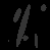
\includegraphics[width=0.27\linewidth]{images/grayscalesample.png}
   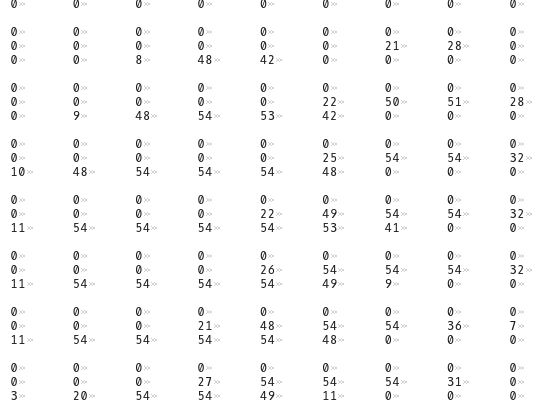
\includegraphics[width=0.47\linewidth]{images/imArraypart.png} \\
   
   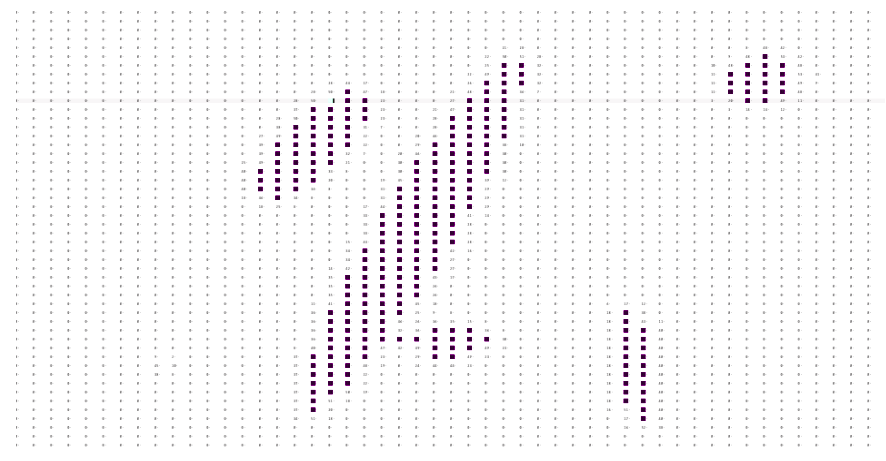
\includegraphics[width=0.67\linewidth]{images/imArrayfull.png} \hfill
   \caption[Reading raw data from image]{Reading raw data from image. (a) Original greyscale image (b) A view of raw data array (c) The entire raw data array with main color highlighted}
   \label{fig:rawImage}
\end{figure}

The only problem could comes from the different image formats existing for these purposes; however the software resolved it using \texttt{ImageMagick}, a popular image processing library that can manage a huge number of different formats. The second step is trivial too and can be solved with a simple image processing library (as the previously cited \texttt{ImageMagick}).\\

In next sections we will see in detail the remaining steps which are also the more interesting.

\section{Images resizing}\label{sec32:ImagesResizing}

A functionality that can be useful when dealing with medical images is image resizing. In fact we often have images larger than the parts we are interested in, so we can gain a great speedup with removal of useless data. Moreover, how we will see next, the boundary operator depends on the size of a single block which in turn depends on the size of images. So sometimes we would to increase the image dimension, in order to better divide the image into blocks and use a particular boundary operator matrix.\\

When the user wants to resize an image, passes to the software the list of desired boundaries: \textit{[[xcropStart,xcropEnd], [ycropStart,ycropEnd], [zcropStart,zcropEnd]]}. For now we can focus on resizes on x and y axis. In Figure~\ref{fig:resizeCases} we can see some resize cases.

\begin{figure}[htbp] %  figure placement: here, top, bottom
   \centering
   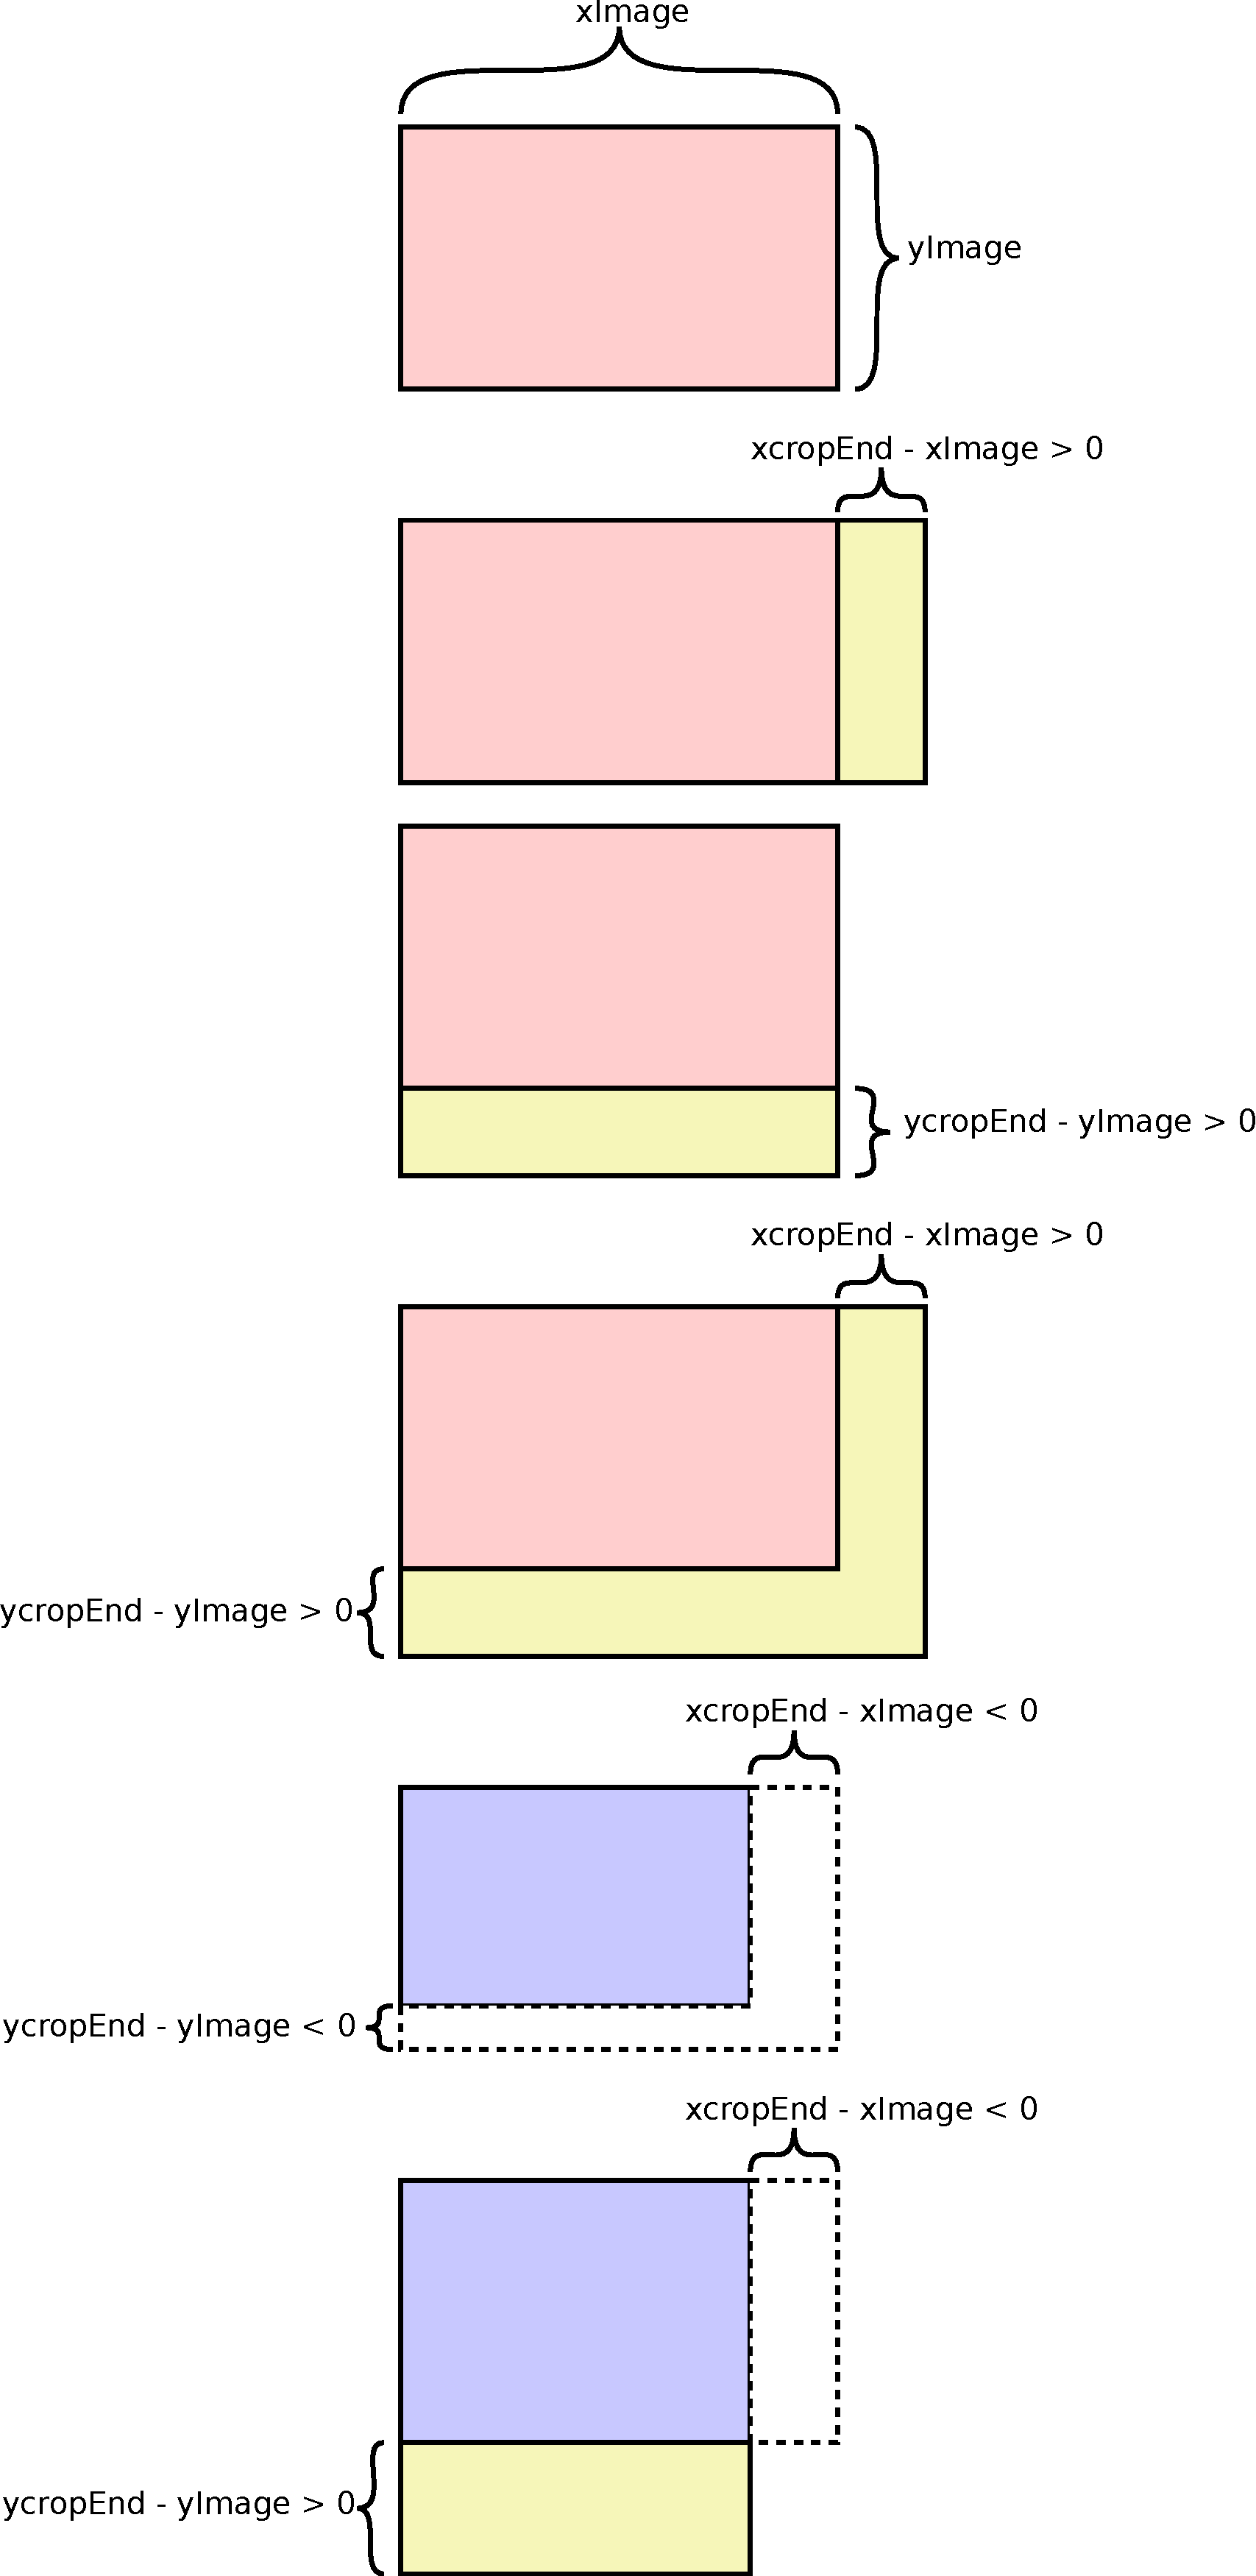
\includegraphics[width=8.5cm]{images/resizeCases.pdf} \hfill
   \caption[Some interesting resize cases]{Some interesting resize cases. (a) The original image (b) Extension on the x dimension (c) Extension on the y dimension (d) Extension on both dimensions (e) Crop of both x and y (f) Crop of x and extension of y}
   \label{fig:resizeCases}
\end{figure}

Reducing dimensions of image is very simple; we just need to load the raw data and select only a slice. Instead, for image extension we need to concatenate rows and columns containing only zero values. This means that the increment of data does not imply an increment of sizes for the final model, as empty zones are not represented.\\

On the z axis the algorithm used is quite different. In fact the z-dimension is determined by the number of images. When we want to reduce the stack we just need to remove images, when we want to increase the stack dimension we just need to add black images at the end.

\section{Creating binary images}\label{sec32:BinaryImages}

When converting from the two-dimensional representation with images to the three-dimensional model, we need binary images. We need this format because we have to be able to unequivocally recognize what to represent in the final result and what we can safely remove. However, we know that in a common medical image every pixel represent a grayscale value and in general we can have several different values. So we need algorithms for mapping of many values into two values, say $0x00$ and $0xff$. 
Moreover, as we can read in \cite{Birkfellner}, physical properties of tissues as recorded by medical imaging devices, do not correlate completely with the anatomic boundaries of certain organs. The problem of the identification of certain regions in an image, is very common in medical imaging processing field and it is referred to as \textbf{segmentation}. So we can use segmentation techniques to find only the right regions for our model contemporary creating binary images.\\

The most basic approach, and the one we will see here, is to divide the image in areas that contain interesting information and areas that are not interesting by making a binary classification based on gray levels. For example from Table~\ref{tbl:Hounsfield} we can see that bones usually have an image density $\rho$ above 50 HU. So we can set a \textbf{threshold} in order to save only pixels that have $\rho$ greater than that value. In Listing~\ref{lst:Thresholding} we have the implementation of the thresholding algorithm for our images

\begin{pseudo}[caption={Image Thresholding}, label={lst:Thresholding}]
begin
 for i in length($image$):
   for j in length($image$[0]):
     if $image$[i][j] > threshold:
       $image$[i][j] = $0xff$
     else:
       $image$[i][j] = $0x00$
 return $image$
end       
\end{pseudo}

However, if the user does not want to set a threshold (or he does not know a value for it), can create the binary images by using \textbf{clustering}. This is a definition for clustering (taken from Wikipedia):
\begin{definition}[Clustering]
 The clustering is the task of grouping a set of objects in such a way that objects in the same group (called a \textbf{cluster}) are more similar (in some sense or another) to each other than to those in other groups (clusters).
\end{definition}

So the clustering is not one specific algorithm but the task to be solved. It can be achieved by many algorithm but here we will see only the \textbf{k-mean algorithm}. Here, we have a set of \textit{observations} $(x_1,x_2,\dots,x_n)$, where each observation is a d-dimensional real vector. We want to partition the $n$ observations into $k \leq n$ sets $S = \{S_1,S_2,\dots,S_k \}$ in order to minimize the within-cluster sum of square distances. In Listing~\ref{lst:kmeans} there is the pseudocode:

\begin{pseudo}[caption={K-means algorithm}, label={lst:kmeans}]
begin
  Initialize cluster centroids $m_1^{(1)},\dots,m_k^{(1)}$
  do until <convergence-condition>:
    $S_i^{(t)} = \{ x_p \colon \| x_p - m^{(t)}_i \|^2 \le \| x_p - m^{(t)}_j \|^2 \ \forall j, 1 \le j \le k \}$
				    \\Assignment step
    $m^{(t+1)}_i = \frac{1}{|S^{(t)}_i|} \displaystyle\sum_{x_j \in S^{(t)}_i} x_j$ \\ Update step
end       
\end{pseudo}

We reach the convergence condition when the assignments no longer changes. In Figure~\ref{fig:kmeans} there is an example of k-means computing.

\begin{figure}[htb] %  figure placement: here, top, bottom
   \centering
   (a)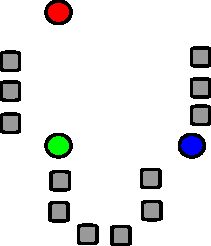
\includegraphics[width=0.20\linewidth]{images/K_Means_Example_Step_1.pdf}\hfill
   (b)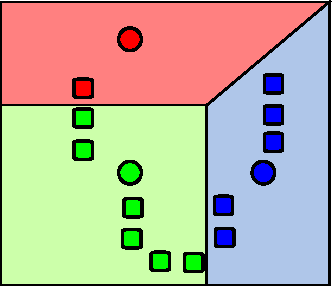
\includegraphics[width=0.20\linewidth]{images/K_Means_Example_Step_2.pdf}\hfill
   (c)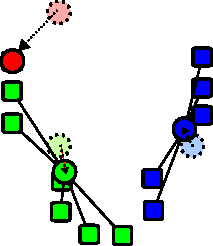
\includegraphics[width=0.20\linewidth]{images/K_Means_Example_Step_3.pdf}\hfill
   (d)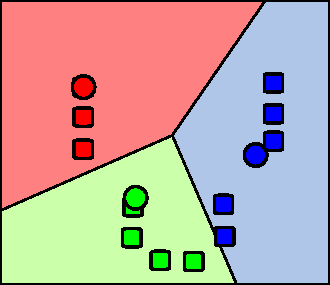
\includegraphics[width=0.20\linewidth]{images/K_Means_Example_Step_4.pdf}
   \caption[K-means clustering]{K-means clustering. (a) k initial "means" (in this case k=3) are randomly generated within the data domain (shown in color). (b) k-clusters are created by associating every observation with the nearest mean. The partitions here represent the Voronoi diagram generated by the means. (c) The centroid of each of the k-clusters becomes the new mean. (d) Steps $b$ and $c$ are repeated until convergence has been reached. Images taken from Wikipedia}
   \label{fig:kmeans}
\end{figure}

In our application, we have only two cluster and we will assign the $0x00$ and $0xff$ values depending on which cluster the pixel are.

\section{Images filtering}\label{sec32:ImagesFiltering}
Now we are interested in improving quality of our images. So for example we have implemented a filter for removal of noise from the image. Our choice fell on a \textbf{median filter}, because it preserves better the image edges. The main idea is to iterate on every pixel of the image replacing each value with the median of neighbors. The pattern of neighbors is called \textbf{window} which slides over the entire image, and we can have a lot of possible patterns (such as boxes or crosses). For a better understanding we can see the following example with a window of size three. Given a one-dimensional vector $x = [4\; 65\; 8\; 3]$, the filtered output $y$ will be:\\
$y[1] = Median[4\; 4\; 65] = 4$\\
$y[2] = Median[4\; 65\; 8] = 8$\\
$y[3] = Median[65\; 8\; 3] = 8$\\
$y[4] = Median[8\; 3\; 3] = 3$\\
So $y = [4\; 8\; 8\; 3]$. How we can see, when we consider the boundaries  we repeat the first or the last value. However other choices are possible, for example we could not consider boundaries or fetching entries for other places. A simple implementation of a median filter is given in Listing~\ref{lst:medianFilter}.

\begin{pseudo}[caption={Median filter}, label={lst:medianFilter}]
begin
  $edge_x = \lfloor(\frac{window\; width}{2})\rfloor$
  $edge_y = \lfloor(\frac{window\; height}{2})\rfloor$
  for $x$ from $edge_x$ to $image\; width - edge_x$:
    for $y$ from $edge_x$ to $image\; height - edge_y$:
      $i = 0$
      for $f_x$ from $0$ to $window\; width$:
        for $f_y$ from $0$ to $window\; height$:
          $window[i] = inputPixelValue[x + f_x - edge_x][y + f_y - edge_y]$
          $i++$
      sort entries in $window$
      $outputPixelValue[x][y] = window[\frac{window\; width \cdot window\; height}{2}]$
  return $outputPixelValue$
end       
\end{pseudo}

However when we have a lot of noise this filter could not work well. In fact, it removes or preserves pixels without seeing if they truly contains a useful information (especially when the noise is concentrated on a big region of the image). So in the software we have implemented a particular filter that consider groups of adjacent pixels on all the stack, removing only ones that have a small size (thus assuming that they are not interesting for our purposes). As a consequence, it is the first part that see our input as a three-dimensional model. The main idea consists in visiting adjacent pixels as they were nodes of a graph using a \textbf{Depth First Search}. The pseudocode is:

\begin{pseudo}[caption={DFS visit}, label={lst:DFS}]
begin
  $S$.push($vertex$) // $S$ is a stack and $v$ is the first vertex
  while $S$ is not empty:
    $v$ = S.pop()
    if $v$ is not labeled as discovered:
      $visited$.push($v$) // $visited$ contains all visited vertices
      label $v$ as discovered
      foreach $edge$ in $adjacentEdges$($v$):
        $S$.push(w)
  return $visited$
end       
\end{pseudo}

The most important part there is the $adjacentEdges$ function, which describes the \textit{adjacency condition} for the given graph and it changes for every particular application. This is a function valid for every type of graph. What can change from an application to another is the \textit{adjacency condition}. The adjacency condition used in this case is trivial. In fact we assume that:
\begin{definition}[Adjacency condition for pixels]
Given a pixel with coordinates (xPixel, yPixel, zPixel) we consider only the following adjacent pixels:
\begin{description}
 \item z $\in$ [zPixel - 1, zPixel + 1]
 \item coordinates = \{(xPixel - 1, yPixel, z), (xPixel + 1, yPixel, z), (xPixel, yPixel - 1, z), (xPixel, yPixel + 1, z)\}
\end{description}
\end{definition}

\begin{figure}[htb]
  \begin{center}
    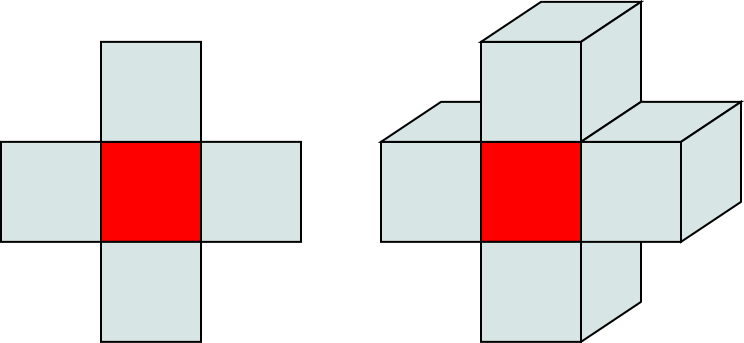
\includegraphics[width=0.60\linewidth]{images/PixelAdjacency.png}
  \end{center}
  \caption[Adjacency relationship for pixels]{Adjacency relationship for pixels. (a) A 2D view of the relationship. (b) A 3D view of the relationship (where the z-axis is determined by previous and next pictures in the array stack}
  \label{fig:pixelAdj}
\end{figure}

Summing up, the code for the three-dimensional filter is the following:

\begin{pseudo}[caption={3D filter}, label={lst:3DFilter}]
begin
  foreach pixel $p$:
    if $p$ was not visited:
      $visited = DFS(p) $
      if $visited$.length < $threshold$:
        mark all pixels in $visited$ as $0x00$
      mark all nodes in $visited$ as visited
end       
\end{pseudo}